\documentclass[10pt]{article}
\usepackage[ngerman]{babel}
\usepackage[utf8]{inputenc}
\usepackage[T1]{fontenc}
\usepackage{amsmath}
\usepackage{amsfonts}
\usepackage{amssymb}
\usepackage[version=4]{mhchem}
\usepackage{stmaryrd}
\usepackage{graphicx}
\usepackage[export]{adjustbox}
\graphicspath{ {./images/} }
\usepackage{bbold}

\title{Hauptprüfung Abiturprüfung 2022 - Leistungsfach }

\author{Alexander Schwarz\\
www.mathe-aufgaben.com}
\date{}


\begin{document}
\maketitle
 Baden-Württemberg\section*{Pflichtteil - Aufgabensatz 2 \\
 Hilfsmittel: keine allgemeinbildende Gymnasien }
Juni 2022

\section*{Aufgabe 1: (2,5 VP)}
Gegeben ist die Funktion $f$ mit $f(x)=e^{0,5 x^{2}}$.\\
Bestimmen Sie den Wert der zweiten Ableitung von $f$ an der Stelle $x_{0}=0$.

\section*{Aufgabe 2: (0,5 VP und 2 VP)}
Abgebildet sind die Graphen der Funktionen f und $g$ mit\\
$f(x)=4-3 x^{2}$ und $g(x)=\sin \left(\frac{\pi}{2} x\right)$.\\
a) Zeigen Sie, dass sich die beiden Graphen an der Stelle $\mathrm{x}_{0}=1$ schneiden.\\
b) Berechnen Sie den Inhalt der markierten Fläche.\\
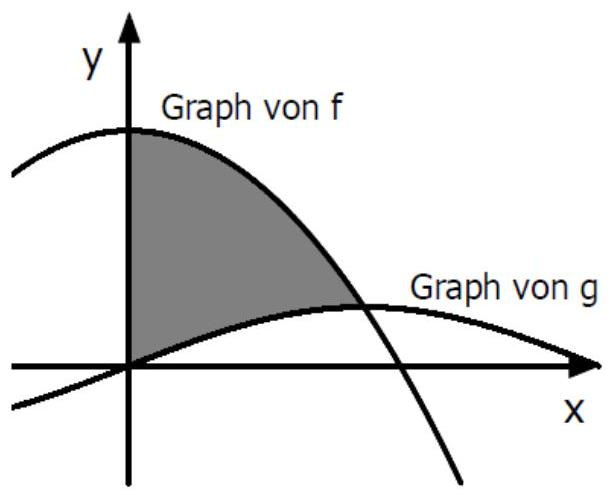
\includegraphics[max width=\textwidth, center]{2025_04_24_60f0811a423d4ef3594fg-2}

\section*{Aufgabe 3: (2,5 VP)}
Der Graph $G_{f}$ der Funktion $f$ besitzt den Tiefpunkt T(1|-2). Der Graph der Funktion g mit $g(x)=\frac{1}{9} x^{3}-3 x$ entsteht, indem $G_{f}$ um a Einheiten nach rechts und um $b$ Einheiten nach unten verschoben wird. Bestimmen Sie die Werte von a und b.

\section*{Aufgabe 4: (2,5 VP)}
Die Graphen einer Schar ganzrationaler Funktionen dritten Grades berühren die $x$-Achse im Punkt $\mathrm{O}(0 \mid 0)$. Jeder Graph der Schar besitzt die Extremstelle $\mathrm{x}_{0}=-2$. Untersuchen Sie, ob alle Graphen der Schar den Punkt P(-3|0) gemeinsam haben.

\section*{Aufgabe 5: (1 VP und 1,5 VP)}
Gegeben sind die Ebene $E: 2 x_{1}+3 x_{2}-4 x_{3}=12$ und für jedes $a \in \mathbb{R}$ eine Gerade $g_{a}: \vec{x}=\left(\begin{array}{c}-1 \\ 5 \\ 3\end{array}\right)+t \cdot\left(\begin{array}{c}a \\ -5 \\ -4\end{array}\right), t \in \mathbb{R}$.\\
a) Bestimmen Sie den Wert von a, für den die Gerade $g_{a}$ parallel zu $E$ ist.\\
b) Für jedes $\mathrm{a} \in \mathbb{R}$ ist $P_{a}$ der Schnittpunkt von $g_{a}$ mit der $x_{1} x_{3}$-Ebene.

Bestimmen Sie den Wert von $a$, für den $P_{a}$ in $E$ liegt.

\section*{Aufgabe 6: (1 VP und 1,5 VP)}
Gegeben sind die parallelen Geraden\\
$g: \vec{x}=\left(\begin{array}{c}6 \\ 5 \\ -2\end{array}\right)+s \cdot\left(\begin{array}{c}1 \\ 4 \\ -1\end{array}\right), s \in \mathbb{R}$ und $h: \vec{x}=\left(\begin{array}{c}0 \\ -1 \\ 4\end{array}\right)+t \cdot\left(\begin{array}{c}1 \\ 4 \\ -1\end{array}\right), t \in \mathbb{R}$.\\
a) Der Punkt $A(4|-3| 0)$ liegt auf $g$. Weisen Sie nach, dass A derjenige Punkt auf $g$ ist, der vom Punkt $\mathrm{B}(0|-1| 4)$ den kleinsten Abstand hat.\\
b) Die Gerade h ist die Bildgerade von g bei einer Spiegelung an der Ebene E . Ermitteln Sie eine Gleichung von E.

\section*{Aufgabe 7: (1 VP und 1,5 VP)}
Ein Glücksrad besteht aus einem gelben, einem blauen und einem roten Sektor. Wird das Glücksrad einmal gedreht, erscheint der gelbe Sektor mit der Wahrscheinlichkeit $\frac{1}{3}$ und der rote Sektor mit der Wahrscheinlichkeit $\frac{1}{2}$.\\
a) Berechnen Sie die Wahrscheinlichkeit dafür, dass bei zweimaligem Drehen der blaue Sektor zweimal erscheint.\\
b) Beschreiben Sie im Sachzusammenhang ein Zufallsexperiment und ein Ereignis, dessen Wahrscheinlichkeit sich mit dem Term $\left(\frac{1}{3}\right)^{5}+5 \cdot\left(\frac{1}{3}\right)^{4} \cdot \frac{2}{3}$ berechnen lässt.

\section*{Aufgabe 8: (1 VP und 1,5 VP)}
Gegeben sind die im Folgenden beschriebenen Zufallsgrößen X und Y :

\begin{itemize}
  \item Ein Würfel, dessen Seiten mit den Zahlen von 1 bis 6 durchnummeriert sind, wird zweimal geworfen. X gibt die Summe der dabei gewürfelten Zahlen an.
  \item Aus einem Behälter mit 60 schwarzen und 40 weißen Kugeln wird zwölfmal nacheinander jeweils eine Kugel zufällig entnommen und wieder zurückgelegt. Y gibt die Anzahl der entnommenen schwarzen Kugeln an.\\
a) Begründen Sie, dass die Wahrscheinlichkeit $\mathrm{P}(\mathrm{X}=4)$ mit der Wahrscheinlichkeit $P(X=10)$ übereinstimmt.\\
b) Die Wahrscheinlichkeitsverteilungen von $X$ und $Y$ werden jeweils durch eines der folgenden Diagramme I, II und III dargestellt. Ordnen Sie $X$ und $Y$ jeweils dem passenden Diagramm zu und begründen Sie Ihre Zuordnung.\\
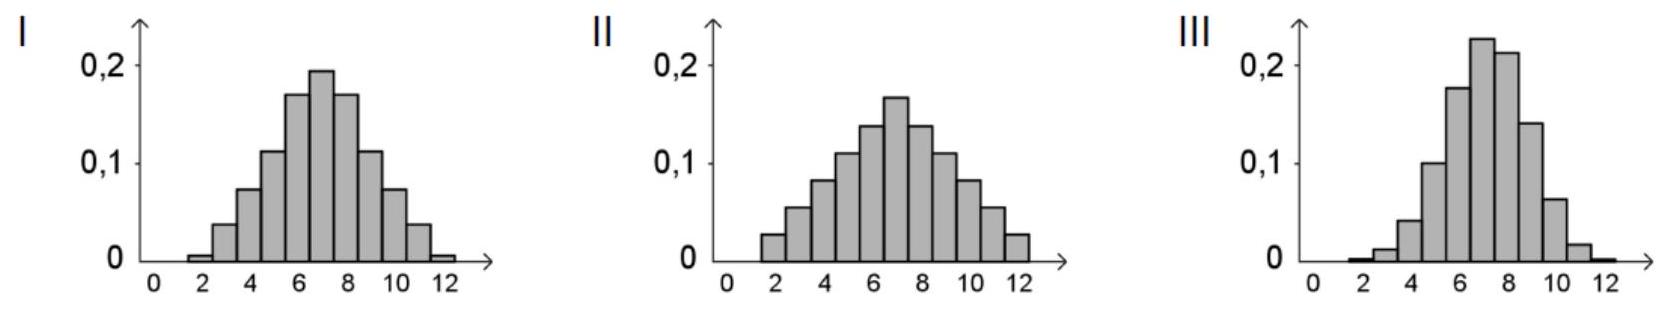
\includegraphics[max width=\textwidth, center]{2025_04_24_60f0811a423d4ef3594fg-4}
\end{itemize}

\section*{Lösungen}
\section*{Aufgabe 1:}
Gegeben ist die Funktion $f(x)=e^{0,5 x^{2}}$\\
1.Ableitung (Kettenregel): $f^{\prime}(x)=e^{0,5 x^{2}} \cdot x$\\
2.Ableitung (Produkt- und Kettenregel): $f^{\prime \prime}(x)=e^{0,5 x^{2}} \cdot x \cdot x+e^{0,5 x^{2}}=e^{0,5 x^{2}} \cdot\left(x^{2}+1\right)$ $f^{\prime \prime}(0)=e^{0} \cdot(0+1)=1$

\section*{Aufgabe 2:}
a) Es gilt $f(1)=4-3 \cdot 1^{2}=1$ und $g(1)=\sin \left(\frac{\pi}{2}\right)=1$.

Da $f(1)=g(1)$ gilt, schneiden sich die Schaubilder an der Stelle $x=1$.\\
b) Berechnung des Flächeninhalts:

$$
\begin{aligned}
A & =\int_{0}^{1}(f(x)-g(x)) d x=\int_{0}^{1}\left(4-3 x^{2}-\sin \left(\frac{\pi}{2} x\right)\right) d x=\left[4 x-x^{3}+\cos \left(\frac{\pi}{2} x\right) \cdot \frac{2}{\pi}\right]_{0}^{1} \\
& =4-1+0-\left(0-0+1 \cdot \frac{2}{\pi}\right)=3-\frac{2}{\pi}
\end{aligned}
$$

\section*{Aufgabe 3:}
Berechnung des Tiefpunktes des Schaubildes der Funktion $g(x)=\frac{1}{9} x^{3}-3 x$ :\\
Bedingung: $g^{\prime}(x)=0$ und $g^{\prime \prime}(x)>0$\\
Es gilt $g^{\prime}(x)=\frac{1}{3} x^{2}-3$ und $g^{\prime \prime}(x)=\frac{2}{3} x$.\\
$\frac{1}{3} x^{2}-3=0 \Leftrightarrow x^{2}=9 \Rightarrow x= \pm 3$\\
$\mathrm{g}^{\prime \prime}(-3)=-2<0 \Rightarrow$ lokales Maximum\\
$\mathrm{g}^{\prime \prime}(3)=2>0 \Rightarrow$ lokales Minimum, also existiert bei $\mathrm{x}=3$ ein Tiefpunkt.\\
Wegen $g(3)=-6$ hat der Tiefpunkt die Koordinaten $T_{g}(3 \mid-6)$.\\
Da das Schaubild von $f$ den Tiefpunkt T(1|-2) besitzt, muss das Schaubild von $f$ um 2 Einheiten nach rechts und um 4 Einheiten nach unten verschoben wird.\\
Daher ist $\mathrm{a}=2$ und $\mathrm{b}=4$.

\section*{Aufgabe 4:}
Ansatz für die Funktionsgleichung: $f(x)=a x^{3}+b x^{2}+c x+d$\\
Es gilt $f^{\prime}(x)=3 a x^{2}+2 b x+c$\\
Bedingung:\\
$O(0 \mid 0)$ liegt auf dem Schaubild: $f(0)=0: d=0$\\
Berührung in $O(0 \mid 0): f^{\prime}(0)=0: c=0$\\
Extremstelle $x_{0}=-2: f^{\prime}(-2)=0: 12 a-4 b+c=0$\\
Da $c=d=0$ ist bleibt als Gleichung 12a $-4 b=0$ übrig.\\
Daraus folgt $b=3 a$.\\
Die Funktionsgleichung mit dem Scharparameter a ausgedrückt werden: $f(x)=a x^{3}+3 \mathrm{ax}^{2}$

Kontrolle, ob P(-3|0) auf allen Graphen der Schar liegen: $f(-3)=0$.

\section*{Aufgabe 5:}
a) Die Gerade $\mathrm{g}_{\mathrm{a}}$ ist parallel zu E, wenn der Richtungsvektor der Geraden orthogonal zum Normalenvektor von E ist.

Bedingung: $\left(\begin{array}{c}a \\ -5 \\ -4\end{array}\right) \cdot\left(\begin{array}{c}2 \\ 3 \\ -4\end{array}\right)=0 \Leftrightarrow 2 a-15+16=0 \Leftrightarrow a=-0,5$\\
b) Der Schnittpunkt von $\mathrm{g}_{\mathrm{a}}$ mit der $\mathrm{x}_{1} \mathrm{x}_{3}$-Ebene hat die Struktur $\left(\mathrm{x}_{1}|0| \mathrm{x}_{3}\right)$

Einsetzen in die Geradengleichung: $\left(\begin{array}{c}x_{1} \\ 0 \\ x_{3}\end{array}\right)=\left(\begin{array}{c}-1 \\ 5 \\ 3\end{array}\right)+t \cdot\left(\begin{array}{c}a \\ -5 \\ -4\end{array}\right)$\\
Aus der 2.Zeile folgt $0=5-5 t \Leftrightarrow t=1$\\
Daraus folgt $x_{1}=-1+a$ und $x_{3}=-1$.\\
Der Schnittpunkt hat die Koordinaten $\mathrm{P}_{\mathrm{a}}(-1+\mathrm{a}|0|-1)$.\\
Einsetzen von $P_{a}$ in $E: 2 \cdot(-1+a)+3 \cdot 0-4 \cdot(-1)=12$

$$
-2+2 a+4=12 \Leftrightarrow a=5
$$

Der gesuchte Wert ist $\mathrm{a}=5$.

\section*{Aufgabe 6:}
a) Der Punkt $\mathrm{A}(4|-3| 0)$ auf $g$ hat vom Punkt $\mathrm{B}(0|-1| 4)$ den kleinsten Abstand, wenn der Vektor $\overrightarrow{\mathrm{AB}}=\left(\begin{array}{c}-4 \\ 2 \\ 4\end{array}\right)$ senkrecht auf der Gerade $g$ (also auf dem Richtungsvektor von g) steht.

Kontrolle: $\left(\begin{array}{c}-4 \\ 2 \\ 4\end{array}\right) \cdot\left(\begin{array}{c}1 \\ 4 \\ -1\end{array}\right)=-4+8-4=0$ was zu zeigen war\\
b) Die Geraden g und h sind parallel.

Skizze unter Einbezug der Informationen aus a):\\
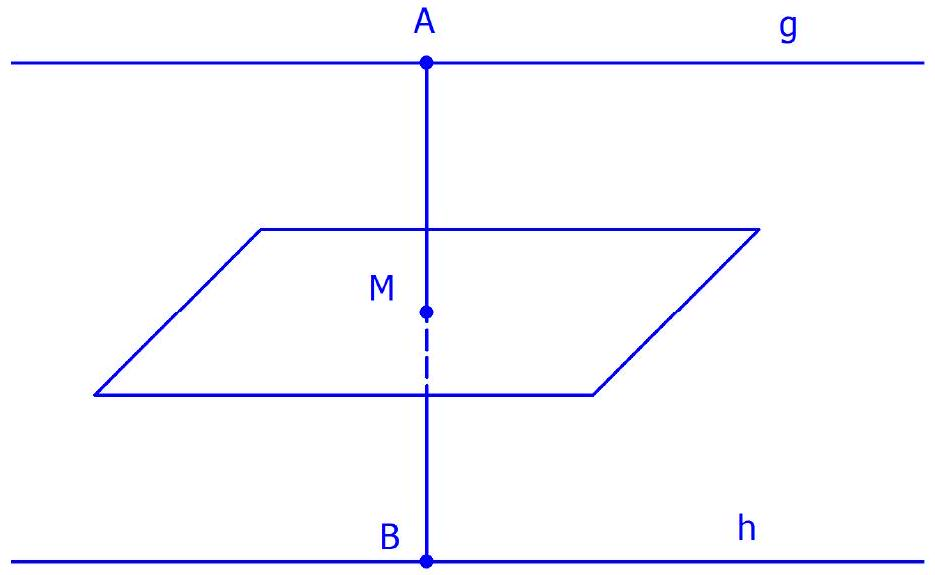
\includegraphics[max width=\textwidth, center]{2025_04_24_60f0811a423d4ef3594fg-7}

Der Mittelpunkt $M$ der Strecke $\overline{\mathrm{AB}}$ liegt auf der Ebene: $M\left(\frac{4+0}{2}\left|\frac{-3-1}{2}\right| \frac{0+4}{2}\right)$, also $M(2|-2| 2)$

Normalenvektor von $\mathrm{E}: \overrightarrow{\mathrm{AB}}=\left(\begin{array}{c}-4 \\ 2 \\ 4\end{array}\right)$\\
Koordinatengleichung von $E:-4 x_{1}+2 x_{2}+4 x_{3}=d$\\
Einsetzen von M ergibt $-8-4+8=\mathrm{d}$, also $\mathrm{d}=-4$.\\
E: $-4 x_{1}+2 x_{2}+4 x_{3}=-4$

\section*{Aufgabe 7:}
a) Die Wahrscheinlichkeit für den blauen Sektor beträgt $1-\frac{1}{2}-\frac{1}{3}=\frac{1}{6}$. $P(b b)=\frac{1}{6} \cdot \frac{1}{6}=\frac{1}{36}$\\
b) Der Term $\left(\frac{1}{3}\right)^{5}$ gibt die Wahrscheinlichkeit an, dass man bei fünfmaligem Drehen 5 mal der gelbe Sektor erscheint.

Der Term $5 \cdot\left(\frac{1}{3}\right)^{4} \cdot \frac{2}{3}$ gibt die Wahrscheinlichkeit an, dass man bei fünfmaligem Drehen 4mal der gelbe Sektor erscheint (Bernoulli-Formel).

Fazit: Der angegebene Term gibt die Wahrscheinilchkeit an, dass man bei fünfmaligem Drehen mindestens 4 mal der gelbe Sektor erscheint.

\section*{Aufgabe 8:}
a) $P(X=4)$ ist die Wahrscheinlichkeit dafür, dass die Summe der gewürfelten Zahlen 4 beträgt.\\
Die Summe 4 ergibt sich für die drei Kombinationen 13, 22 und 31.\\
Somit ist die Wahrscheinlichkeit $P(X=4)=\frac{3}{36}$.\\
$P(X=10)$ ist die Wahrscheinlichkeit dafür, dass die Summe der gewürfelten Zahlen 10 beträgt.\\
Die Summe 10 ergibt sich für die drei Kombinationen 46, 55 und 64.\\
Somit ist die Wahrscheinlichkeit $P(X=10)=\frac{3}{36}$.\\
b) Die Zufallsgröße $Y$ ist binomialverteilt mit $n=12$ und $p=\frac{60}{100}=0,6$.

Da $p \neq 0,5$ ist, ist die Verteilung von $Y$ nicht symmetrisch.\\
Somit kommt nur das Diagramm III in Frage.\\
Die Wahrscheinlichkeitsverteilung von X ist symmetrisch.\\
Die größte Wahrscheinlichkeit ist $P(X=7)=\frac{6}{36}=\frac{1}{6}$, da folgende Kombinationen die Summe 7 ergeben: 16, 25, 34, 43, 52, 61

Da $\frac{1}{6} \approx 0,167$ ist, gehört Diagramm II zu X.\\
Bei Diagramm I besitzt die Säule an der Stelle X=7 eine Wahrscheinlichkeit von 0,2.

Andere Begründung:\\
Es gilt $P(X=2)=\frac{1}{36}$ (wenn 11 gewürfelt wird) und $P(X=3)=\frac{2}{36}$ (wenn 12 oder 21 gewürfelt wird).\\
Die Wahrscheinlichkeit $P(X=3)$ ist daher doppelt so groß wie $P(X=2)$, was bei Diagramm II passt und bei Diagramm I nicht.


\end{document}